% Practice Test 14 — Florida Edition
% Questions: 30 (21 MC + 9 SA)
% Generated by scripts/generate_practice_tests.py

\begin{practiceQuestion}{1-3-q02}{mc}
\begin{questionText}
In a proportional relationship, the constant of proportionality $k$ equals:
\end{questionText}
\choiceA{$x \div y$}
\choiceB{$y \div x$}
\choiceC{$x \times y$}
\choiceD{$y - x$}
\correctAnswer{B}
\explanation{The constant of proportionality is $k = \frac{y}{x}$, which is the unit rate.}
\end{practiceQuestion}

\begin{practiceQuestion}{1-6-q22}{sa}
\begin{questionText}
Brand A juice: $32$ oz for $\$2.56$. Brand B juice: $48$ oz for $\$3.60$. Which brand has the better price per ounce, and what is it?
\end{questionText}
\correctAnswer{Brand B at $\$0.075$ per oz}
\explanation{A: $2.56 \div 32 = \$0.08$/oz. B: $3.60 \div 48 = \$0.075$/oz. Brand B is cheaper per ounce.}
\end{practiceQuestion}

\begin{practiceQuestion}{2-1-q08}{mc}
\begin{questionText}
$36$ is $45\%$ of what number?
\end{questionText}
\choiceA{$16.2$}
\choiceB{$72$}
\choiceC{$80$}
\choiceD{$90$}
\correctAnswer{C}
\explanation{Divide the part by the percent: $36 \div 0.45 = 80$.}
\end{practiceQuestion}

\begin{practiceQuestion}{2-2-q29}{gsa}
\begin{questionText}
The double number line below shows a percent relationship. What number goes at the question mark?

\begin{center}
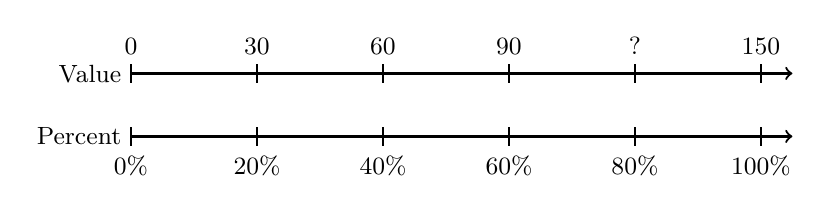
\begin{tikzpicture}[scale=0.8]
  % Top number line (values)
  \draw[thick,->] (0,1) -- (10.5,1);
  \node[left,font=\small] at (0,1) {Value};
  \foreach \x/\lab in {0/0, 2/30, 4/60, 6/90, 8/?, 10/150} {
    \draw[thick] (\x,0.85) -- (\x,1.15);
    \node[above,font=\small] at (\x,1.15) {\lab};
  }
  % Bottom number line (percent)
  \draw[thick,->] (0,0) -- (10.5,0);
  \node[left,font=\small] at (0,0) {Percent};
  \foreach \x/\lab in {0/0\%, 2/20\%, 4/40\%, 6/60\%, 8/80\%, 10/100\%} {
    \draw[thick] (\x,-0.15) -- (\x,0.15);
    \node[below,font=\small] at (\x,-0.15) {\lab};
  }
\end{tikzpicture}
\end{center}
\end{questionText}
\correctAnswer{$120$}
\explanation{The whole ($100\%$) corresponds to $150$. At $80\%$: $\frac{n}{150} = \frac{80}{100}$ → $n = 120$.}
\end{practiceQuestion}

\begin{practiceQuestion}{2-6-q29}{gsa}
\begin{questionText}
The line graph shows the growth of a $\$1{,}200$ deposit at simple interest. How much interest was earned from Year $0$ to Year $4$?

\begin{center}
\begin{tikzpicture}[scale=0.7]
  \draw[thick,->] (0,0) -- (5.5,0) node[right]{\small Years};
  \draw[thick,->] (0,0) -- (0,5.5) node[above]{\small Total (\$)};
  \draw[gray!20,thin] (0,0) grid[step=1] (5,5);
  \foreach \x in {0,...,4} {
    \node[below,font=\small] at (\x,0) {$\x$};
  }
  \foreach \y/\lab in {1/300,2/600,3/900,4/1200,5/1500} {
    \draw (-0.1,\y) -- (0.1,\y) node[left,font=\small,xshift=-2pt] {\lab};
  }
  % P = 1200, r = 5%, I/year = 60
  % t=0:1200, t=1:1260, t=2:1320, t=3:1380, t=4:1440
  \filldraw[funBlue] (0,4) circle (3pt);
  \filldraw[funBlue] (1,4.2) circle (3pt);
  \filldraw[funBlue] (2,4.4) circle (3pt);
  \filldraw[funBlue] (3,4.6) circle (3pt);
  \filldraw[funBlue] (4,4.8) circle (3pt);
  \draw[thick,funBlue] (0,4) -- (1,4.2) -- (2,4.4) -- (3,4.6) -- (4,4.8);
  \node[above left,font=\small] at (0,4) {$\$1{,}200$};
  \node[above right,font=\small] at (4,4.8) {$\$1{,}440$};
\end{tikzpicture}
\end{center}
\end{questionText}
\correctAnswer{$\$240$}
\explanation{Interest $= 1{,}440 - 1{,}200 = \$240$.}
\end{practiceQuestion}

\begin{practiceQuestion}{2-7-q20}{sa}
\begin{questionText}
A student predicted a plant would grow $15$ cm. It actually grew $12$ cm. What is the percent error?
\end{questionText}
\correctAnswer{$25\%$}
\explanation{$\frac{|15 - 12|}{12} \times 100 = \frac{3}{12} \times 100 = 25\%$.}
\end{practiceQuestion}

\begin{practiceQuestion}{3-2-q22}{sa}
\begin{questionText}
What is $(-18) + 18$?
\end{questionText}
\correctAnswer{$0$}
\explanation{$-18$ and $18$ are additive inverses (opposites). Their sum is always $0$.}
\end{practiceQuestion}

\begin{practiceQuestion}{3-3-q24}{sa}
\begin{questionText}
Evaluate: $15 - 22 - (-4)$.
\end{questionText}
\correctAnswer{$-3$}
\explanation{$15 - 22 = 15 + (-22) = -7$. Then $-7 - (-4) = -7 + 4 = -3$.}
\end{practiceQuestion}

\begin{practiceQuestion}{4-4-q18}{mc}
\begin{questionText}
Which shows the correct way to check that $4(3n - 2) = 12n - 8$?
\end{questionText}
\choiceA{Add $3n$ and $-2$ to get $n$, then multiply by $4$}
\choiceB{Expand: $4 \times 3n = 12n$ and $4 \times (-2) = -8$, so $12n - 8$}
\choiceC{Divide $12n$ by $4$ and $-8$ by $3$}
\choiceD{Substitute $n = 0$: $4(3(0) - 2) = 4(-2) = 8$}
\correctAnswer{B}
\explanation{To check factoring, expand by distributing $4$ to each term inside: $4 \times 3n = 12n$ and $4 \times (-2) = -8$. This gives $12n - 8$, confirming the factoring.}
\end{practiceQuestion}

\begin{practiceQuestion}{4-5-q17}{mc}
\begin{questionText}
Which expression is equivalent to $(2x - 5) + (x + 8) - (3x - 2)$?
\end{questionText}
\choiceA{$5$}
\choiceB{$6x + 5$}
\choiceC{$-1$}
\choiceD{$6x + 1$}
\correctAnswer{A}
\explanation{Combine: $2x - 5 + x + 8 - 3x + 2$. Variable: $2x + x - 3x = 0$. Constants: $-5 + 8 + 2 = 5$.}
\end{practiceQuestion}

\begin{practiceQuestion}{5-3-q07}{mc}
\begin{questionText}
Solve $3(2x + 1) = 21$.
\end{questionText}
\choiceA{$x = 3$}
\choiceB{$x = 6$}
\choiceC{$x = 10$}
\choiceD{$x = \dfrac{20}{6}$}
\correctAnswer{A}
\explanation{Distribute: $6x + 3 = 21$. Subtract $3$: $6x = 18$. Divide by $6$: $x = 3$. Check: $3(2 \cdot 3 + 1) = 3(7) = 21$ \checkmark.}
\end{practiceQuestion}

\begin{practiceQuestion}{5-4-q06}{mc}
\begin{questionText}
Solve $-0.4y + 2 = 6$.
\end{questionText}
\choiceA{$y = 10$}
\choiceB{$y = -10$}
\choiceC{$y = 20$}
\choiceD{$y = -20$}
\correctAnswer{B}
\explanation{Subtract $2$: $-0.4y = 4$. Divide by $-0.4$: $y = -10$. Check: $-0.4(-10) + 2 = 4 + 2 = 6$ \checkmark.}
\end{practiceQuestion}

\begin{practiceQuestion}{5-5-q28}{gmc}
\begin{questionText}
A store sign shows the rule below. Which inequality represents the sign?

\begin{center}
\begin{tikzpicture}[scale=0.8]
  \draw[thick,rounded corners,fill=funBlue!10] (-0.5,-1.5) rectangle (7,1.5);
  \node[align=center,font=\large] at (3.25,0.4) {\textbf{SALE!}};
  \node[align=center] at (3.25,-0.5) {All items plus $\$5$ tax};
  \node[align=center] at (3.25,-1) {must be \textbf{under} $\$50$};
\end{tikzpicture}
\end{center}

Let $p$ be the price of an item before tax.
\end{questionText}
\choiceA{$p + 5 > 50$}
\choiceB{$p + 5 \leq 50$}
\choiceC{$p + 5 < 50$}
\choiceD{$p + 5 \geq 50$}
\correctAnswer{C}
\explanation{``Under $\$50$'' means strictly less than $50$: $p + 5 < 50$.}
\end{practiceQuestion}

\begin{practiceQuestion}{5-6-q04}{mc}
\begin{questionText}
Solve $3n - 6 > 0$ and describe the graph.
\end{questionText}
\choiceA{Closed circle at $2$, shade right}
\choiceB{Open circle at $2$, shade right}
\choiceC{Open circle at $2$, shade left}
\choiceD{Closed circle at $-2$, shade right}
\correctAnswer{B}
\explanation{Add $6$: $3n > 6$. Divide by $3$: $n > 2$. Open circle at $2$, shade right.}
\end{practiceQuestion}

\begin{practiceQuestion}{6-2-q01}{mc}
\begin{questionText}
A map uses the scale $1$ cm $= 50$ km. You redraw it at $1$ cm $= 25$ km. A road that is $6$ cm on the original map becomes how long on the new map?
\end{questionText}
\choiceA{$3$ cm}
\choiceB{$6$ cm}
\choiceC{$12$ cm}
\choiceD{$150$ cm}
\correctAnswer{C}
\explanation{Scale ratio: $\frac{50}{25} = 2$. New length: $6 \times 2 = 12$ cm. The new scale is more detailed, so the drawing gets bigger.}
\end{practiceQuestion}

\begin{practiceQuestion}{6-4-q03}{mc}
\begin{questionText}
Can a triangle have angles $50°$, $60°$, and $80°$?
\end{questionText}
\choiceA{Yes, because the angles are all positive}
\choiceB{Yes, because each angle is less than $180°$}
\choiceC{No, because $50 + 60 + 80 = 190 \neq 180$}
\choiceD{No, because the angles are not equal}
\correctAnswer{C}
\explanation{The three angles sum to $190°$, not $180°$. Triangle angles must always sum to exactly $180°$.}
\end{practiceQuestion}

\begin{practiceQuestion}{6-5-q17}{mc}
\begin{questionText}
A triangular prism is sliced with a vertical cut perpendicular to the triangular bases. What shape is the cross-section?
\end{questionText}
\choiceA{Triangle}
\choiceB{Rectangle}
\choiceC{Circle}
\choiceD{Trapezoid}
\correctAnswer{B}
\explanation{A vertical cut perpendicular to the triangular bases of a triangular prism produces a rectangle (the cut goes through the lateral faces).}
\end{practiceQuestion}

\begin{practiceQuestion}{6-6-q26}{gmc}
\begin{questionText}
Two lines intersect as shown. What is the value of $x$?

\begin{center}
\begin{tikzpicture}[scale=0.8]
  \draw[thick] (-3,0) -- (3,0);
  \draw[thick] (-2,-2) -- (2,2);
  \node at (1.5,0.5) {\small $x°$};
  \node at (-1.5,-0.6) {\small $x°$};
  \node at (-1.2,0.8) {\small $135°$};
\end{tikzpicture}
\end{center}
\end{questionText}
\choiceA{$35°$}
\choiceB{$45°$}
\choiceC{$55°$}
\choiceD{$135°$}
\correctAnswer{B}
\explanation{The angle $x°$ and $135°$ are supplementary (they are adjacent on a straight line): $x + 135 = 180$. So $x = 45°$.}
\end{practiceQuestion}

\begin{practiceQuestion}{7-1-q12}{mc}
\begin{questionText}
A clock face is a circle with a radius of $15$ cm. What is the diameter of the clock face?
\end{questionText}
\choiceA{$7.5$ cm}
\choiceB{$15$ cm}
\choiceC{$30$ cm}
\choiceD{$45$ cm}
\correctAnswer{C}
\explanation{$d = 2r = 2 \times 15 = 30$ cm.}
\end{practiceQuestion}

\begin{practiceQuestion}{7-5-q20}{sa}
\begin{questionText}
A cube has a side length of $7$ m. What is its surface area?
\end{questionText}
\correctAnswer{$294$ m$^2$}
\explanation{$SA = 6s^2 = 6 \times 49 = 294$ m$^2$.}
\end{practiceQuestion}

\begin{practiceQuestion}{7-6-q06}{mc}
\begin{questionText}
A rectangular box has a volume of $180$ in$^3$. Its length is $10$ in and width is $6$ in. What is its height?
\end{questionText}
\choiceA{$2$ in}
\choiceB{$3$ in}
\choiceC{$5$ in}
\choiceD{$9$ in}
\correctAnswer{B}
\explanation{$V = lwh$. $180 = 10 \times 6 \times h$. $180 = 60h$. $h = 3$ in.}
\end{practiceQuestion}

\begin{practiceQuestion}{7-7-q22}{sa}
\begin{questionText}
A cylinder has a volume of $502.4$ cm$^3$ and a radius of $4$ cm. What is the height? Use $\pi \approx 3.14$.
\end{questionText}
\correctAnswer{$10$ cm}
\explanation{$502.4 = 3.14 \times 16 \times h = 50.24h$. $h = 502.4 \div 50.24 = 10$ cm.}
\end{practiceQuestion}

\begin{practiceQuestion}{8-1-q28}{gmc}
\begin{questionText}
The table below shows the results of two samples taken from a population of $1{,}000$ students.

\begin{center}
\begin{tabular}{|l|c|c|}
\hline
 & \textbf{Sample 1 (50 students)} & \textbf{Sample 2 (50 students)} \\
\hline
Prefer Math & $18$ & $22$ \\
\hline
Prefer Science & $14$ & $12$ \\
\hline
Prefer English & $10$ & $8$ \\
\hline
Prefer Art & $8$ & $8$ \\
\hline
\end{tabular}
\end{center}

Based on both samples, the best prediction for how many of the $1{,}000$ students prefer math is:
\end{questionText}
\choiceA{$180$}
\choiceB{$220$}
\choiceC{$400$}
\choiceD{$360$}
\correctAnswer{C}
\explanation{Average the two samples: $\frac{18+22}{2} = 20$ out of $50 = 40\%$. Then $40\%$ of $1{,}000 = 400$.}
\end{practiceQuestion}

\begin{practiceQuestion}{8-3-q06}{mc}
\begin{questionText}
Team A's scores: mean $72$, MAD $3$. Team B's scores: mean $74$, MAD $8$. Which team is more consistent?
\end{questionText}
\choiceA{Team A because its MAD is smaller}
\choiceB{Team B because its mean is higher}
\choiceC{Team A because its mean is lower}
\choiceD{Team B because its MAD is larger}
\correctAnswer{A}
\explanation{A smaller MAD means scores are closer to the mean, so Team A is more consistent.}
\end{practiceQuestion}

\begin{practiceQuestion}{8-4-q25}{sa}
\begin{questionText}
Team A: mean $88$, range $12$, MAD $3$. Team B: mean $84$, range $30$, MAD $8$. Which team is stronger overall? Justify your answer using at least two measures.
\end{questionText}
\correctAnswer{Team A — higher mean ($88$ vs.\ $84$) and more consistent (MAD $3$ vs.\ $8$, range $12$ vs.\ $30$)}
\explanation{Team A has a higher center (mean $88$) and less variability (smaller MAD and range), meaning Team A is both better on average and more consistent.}
\end{practiceQuestion}

\begin{practiceQuestion}{8-5-q27}{gmc}
\begin{questionText}
The back-to-back stem-and-leaf plot compares quiz scores for two classes.

\begin{center}
\begin{tabular}{r|c|l}
\textbf{Class A} & \textbf{Stem} & \textbf{Class B} \\
\hline
$5\;\;2$ & $6$ & $3\;\;5\;\;8$ \\
$8\;\;5\;\;3\;\;0$ & $7$ & $2\;\;4\;\;9$ \\
$6\;\;4$ & $8$ & $1\;\;3\;\;5\;\;7$ \\
$2$ & $9$ & $0\;\;5$
\end{tabular}

Key: $5 \mid 7$ means $75$ (Class A) and $7 \mid 2$ means $72$ (Class B)
\end{center}

Which class has a higher median?
\end{questionText}
\choiceA{Class A}
\choiceB{Class B}
\choiceC{They have the same median}
\choiceD{Cannot be determined}
\correctAnswer{B}
\explanation{Class A data ($9$ values): $62, 65, 70, 73, 75, 78, 84, 86, 92$. Median $= 75$. Class B data ($12$ values): $63, 65, 68, 72, 74, 79, 81, 83, 85, 87, 90, 95$. Median $= \frac{79+81}{2} = 80$. Class B has a higher median.}
\end{practiceQuestion}

\begin{practiceQuestion}{8-6-q09}{mc}
\begin{questionText}
In a circle graph, two sectors have angles of $144°$ and $72°$. Together, what percent of the whole do they represent?
\end{questionText}
\choiceA{$50\%$}
\choiceB{$60\%$}
\choiceC{$72\%$}
\choiceD{$80\%$}
\correctAnswer{B}
\explanation{$\frac{144 + 72}{360} = \frac{216}{360} = 0.60 = 60\%$.}
\end{practiceQuestion}

\begin{practiceQuestion}{9-4-q16}{mc}
\begin{questionText}
A game has $4$ outcomes: Win Big, Win Small, Lose Small, Lose Big. The probabilities are $0.05$, $0.25$, $0.45$, and $0.25$. Which outcome is LEAST likely?
\end{questionText}
\choiceA{Win Big}
\choiceB{Win Small}
\choiceC{Lose Small}
\choiceD{Lose Big}
\correctAnswer{A}
\explanation{Win Big has the smallest probability ($0.05$), making it least likely.}
\end{practiceQuestion}

\begin{practiceQuestion}{9-6-q11}{mc}
\begin{questionText}
Two dice are rolled. What is the probability that the sum is even?
\end{questionText}
\choiceA{$\frac{1}{4}$}
\choiceB{$\frac{1}{3}$}
\choiceC{$\frac{1}{2}$}
\choiceD{$\frac{2}{3}$}
\correctAnswer{C}
\explanation{Even sums occur when both dice are even or both are odd. Both even: $3 \times 3 = 9$. Both odd: $3 \times 3 = 9$. Total: $18$ out of $36$. $P = \frac{18}{36} = \frac{1}{2}$.}
\end{practiceQuestion}

\begin{practiceQuestion}{9-7-q03}{mc}
\begin{questionText}
To simulate an event with a $\frac{1}{6}$ probability, which tool would be most appropriate?
\end{questionText}
\choiceA{A coin}
\choiceB{A standard die}
\choiceC{A spinner with $4$ sections}
\choiceD{A bag with $2$ marbles}
\correctAnswer{B}
\explanation{A standard die has $6$ equally likely outcomes, each with probability $\frac{1}{6}$.}
\end{practiceQuestion}
